\documentclass[aspectratio=169]{beamer}
\usepackage[UKenglish]{babel}
\usepackage[T1]{fontenc} % fontenc mit T1 sorgt für richtige Kodierung europäischer Zeichen
\usepackage[utf8]{inputenc} % Eingabezeichensatz: direkte Eingabe von Umlauten usw.
 % Anpassung des Dokumants deutsche Richtlinien

\usepackage{url} %Einbinden von Hyperlinks
\usepackage{mdwlist} % Für Listen ohne Abstand zwischen den Aufzählungspunkten.
\usepackage{paralist} % Ermöglicht Anpassung der Listen, z.B. Wahl des Autfählungszeichens

\usepackage{setspace} % Anpassung des Zeilenabstandes, Befehl muss vor der Berechnung des Satzspiegels gesetzt werden.

\usepackage{varioref} %Querverweise mit Seitenreferenz
\usepackage{fancyref} %Querverweise mit Angabe des Typs
%\usepackage[table,gray]{xcolor} %Zum Deaktivieren von Schattierung -- nur bei Verwendung des Pakets "listings"
\usepackage{booktabs} %Zur eleganten Formatierung von Tabellen
\usepackage{tabularx}
\usepackage[format = plain, textfont = normalfont, labelfont = bf, font = scriptsize, ]{caption}
%\usepackage[table,gray]{xcolor} %Zum Deaktivieren von Schattierung -- nur bei Verwendung des Packets "listings"
%\usepackage{listings} %Zur EInbindung von Quellcode verschiednester Art
%\usepackage[locale=DE]{siunitx} % Korrekte Angabe von Einheiten

\beamertemplatenavigationsymbolsempty

%\setbeamertemplate{footline}[text line]{%
%\parbox{\linewidth}{\vspace*{-8pt}Laser cooling\hfill\insertshortauthor\hfill\insertpagenumber}}

\useoutertheme{infolines}
\usecolortheme{beaver}

\title{F61: NMR--Spectroscopy}
%\subtitle{Seminarvortrag im Rahmen des Fortgeschrittenen-Praktikums}
\author{T. Gierlich und A. Impertro}
\date{}

\newcommand{\err}[2]{( #1 \, \pm \, #2 )}

\begin{document}

\begin{frame}
  \begin{center}
    {\LARGE F61: NMR--Spectroscopy}
    
    \bigskip
    
    {\large T. Gierlich and A. Impertro}
        
    \bigskip
   
    {\large May 26th, 2017}
  \end{center}
\end{frame}

\begin{frame}
	\frametitle{Outline}
  	\tableofcontents
\end{frame}

\section{Introduction and Theoretical Concepts}

\begin{frame}
	\frametitle{Introduction}
	\begin{figure}
		\includegraphics[width=0.5\textwidth]{./Resources/nmr_text.png}
		\label{fig:nmr_text}
	\end{figure}
	\flushleft
	%\begin{itemize}
	%	\item \textbf{Nuclear:} Interaction of the nuclear spin...
	%	\item \textbf{Magnetic:} ...with magnetic fields
	%	\item \textbf{Resonance:} $\rightarrow$ resonant interaction
	%	\item \textbf{Spectroscopy:} Resolve the different signal components
	%\end{itemize}
	\vspace*{-15pt}
	\pause
	\hrulefill
	\vspace*{5pt}
	%\textbf{Applications}
	
	\begin{minipage}[t]{0.48 \textwidth}
		\centering
		\textbf{Detection of substances}
		\begin{figure}
			\includegraphics[height=0.3\textheight]{./Resources/cshift.png}
			\label{fig:cshift}
			\caption{\tiny{Carl Nave, Hyperphysics, hyperphysics.phy-astr.gsu.edu}}
		\end{figure}
	\end{minipage}
	\begin{minipage}[t]{0.48 \textwidth}
		\centering
		\textbf{Multidimensional imaging}
		\begin{figure}
			\includegraphics[height=0.3\textheight]{./Resources/mri_head.jpg}
			\label{fig:mri_head}
			\caption{\tiny{Sierra Vista Diagnostics, svdrads.com}}
		\end{figure}
	\end{minipage}
\end{frame}

\begin{frame}
	\frametitle{Theoretical Concepts - Working Principle}
	
	\begin{minipage}[t]{\textwidth}
		\begin{minipage}[t]{0.3\textwidth}
			\centering
			\begin{figure}
				\includegraphics[height=0.3\textheight]{./Resources/magnetization_components.png}
				\caption{Magnetization}
				\label{fig:mag_components}
			\end{figure}
		\end{minipage}
		\begin{minipage}[t]{0.65\textwidth}
			\begin{itemize}
				\item Nuclei with spin $I$ have a magnetic moment $\mu$
				\item Ensemble of many nuclei: Measurable magnetization $\vec{M}$
				\item Minimal energy $\rightarrow$ Dipole aligned parallel to B-field
				\vspace{10pt}
				\item Ground state $\rightarrow$ $M_{\perp} = 0$
			\end{itemize}
			\vspace*{-5pt}
			\hrulefill
		\end{minipage}
	\end{minipage}
	\pause
	\begin{minipage}[t]{\textwidth}
		\begin{minipage}[t]{0.3\textwidth}
			\centering
			\begin{figure}
				\includegraphics[height=0.3\textheight]{./Resources/larmor_precession.png}
				\caption{Larmor-Precession of $M_{\perp}$}
				\label{fig:larmor}
			\end{figure}
		\end{minipage}
		\begin{minipage}[t]{0.65\textwidth}
			\begin{itemize}
				\item Excited states have a component $M_{\perp} \neq 0$
				\item $M_{\perp}$ precesses around the field lines with the Larmor frequency
				\begin{equation}
					\omega_L = \gamma B_0
				\end{equation}
				\item $\omega_L$ can be measured!				
			\end{itemize}
		\end{minipage}
	\end{minipage}

\end{frame}

\begin{frame}
\frametitle{Theoretical Concepts - Working Principle}
\begin{minipage}[t]{0.65\textwidth}
	\textbf{How can we create an excited state ?}
	\begin{itemize}
		\item An oscillating B-Field $\vec{B}_1$ rotates the magnetization $\vec{M}$ by an angle
		\begin{equation}
		\alpha = \gamma B_1 \Delta t
		\end{equation}
	\end{itemize}
\end{minipage}
\hspace*{10pt}
\begin{minipage}[t]{0.3\textwidth}
	\begin{figure}[H]
		\centering
		\includegraphics[width=\textwidth]{./Resources/hf_pulse.png}
		\caption{Rotation of $M$ due to an HF-Pulse}
	\end{figure}
\end{minipage}

\begin{itemize}
	\pause
	\item By choosing $\Delta t$, we can create:
	\begin{itemize}
		\item A perpendicular magnetization ($90^\circ$-Pulse)
		\item An anti-parallel magnetization ($180^\circ$-Pulse)
	\end{itemize}
\end{itemize}
\end{frame}

\begin{frame}
	\frametitle{Setup and Measurement Principle}
	\begin{figure}[H]
		\centering
		\includegraphics[height=0.7 \textheight]{./Resources/setup.png}
		\caption{\tiny{McGraw Hill Higher Education, mhhe.com}}
	\end{figure}
\end{frame}

\section{Part I: Relaxation Times}

\begin{frame}
	\frametitle{Theory of Relaxation}
	\textbf{Excited states decay into the Ground State on a characteristic timescale.}
	
	The decay is of exponential nature and described in the \textit{Bloch equations:}
	\begin{equation}
	\frac{dM_{\perp}(t)}{dt} = - \frac{M_{\perp}(t)}{T_2}
	\end{equation}
	\begin{equation}
	\frac{dM_{\parallel}(t)}{dt} = - \frac{M_{\parallel}(t) - M_0}{T_1}
	\end{equation}
	
	\begin{itemize}
		\item $T_2$: Spin-Lattice Relaxation
		\item $T_1$: Spin-Spin Relaxation
	\end{itemize}
\end{frame}

\begin{frame}
	\frametitle{$T_2$-Measurement: Spin Echo}
	\begin{minipage}[t]{0.45\textwidth}
		\centering
		\textbf{Spin-Echo principle}
		\begin{figure}
			\includegraphics[height=40mm]{./Resources/spin_ech_schematic.png}
			\caption{Principle of the spin-echo method}
			\label{fig:spinecho_bloch}
		\end{figure}
	\end{minipage}
	\hfill
	\pause
	\begin{minipage}[t]{0.45\textwidth}
		\centering
		\textbf{Pulse sequence}
		\begin{figure}
			\includegraphics[height=40mm]{./Resources/spinecho_osci.jpg}
			\caption{Spin-Echo measurement with $\tau=10ms$}
			\label{fig:spinecho_osci}
		\end{figure}
	\end{minipage}
	\pause
	\begin{itemize}
		\item \textbf{Disadvantage}: Dephasing for long measurement times!
	\end{itemize}
\end{frame}

\begin{frame}
	\frametitle{$T_2$-Measurement: Spin Echo}
	\begin{minipage}[t]{0.45\textwidth}
		\centering
		\begin{figure}
			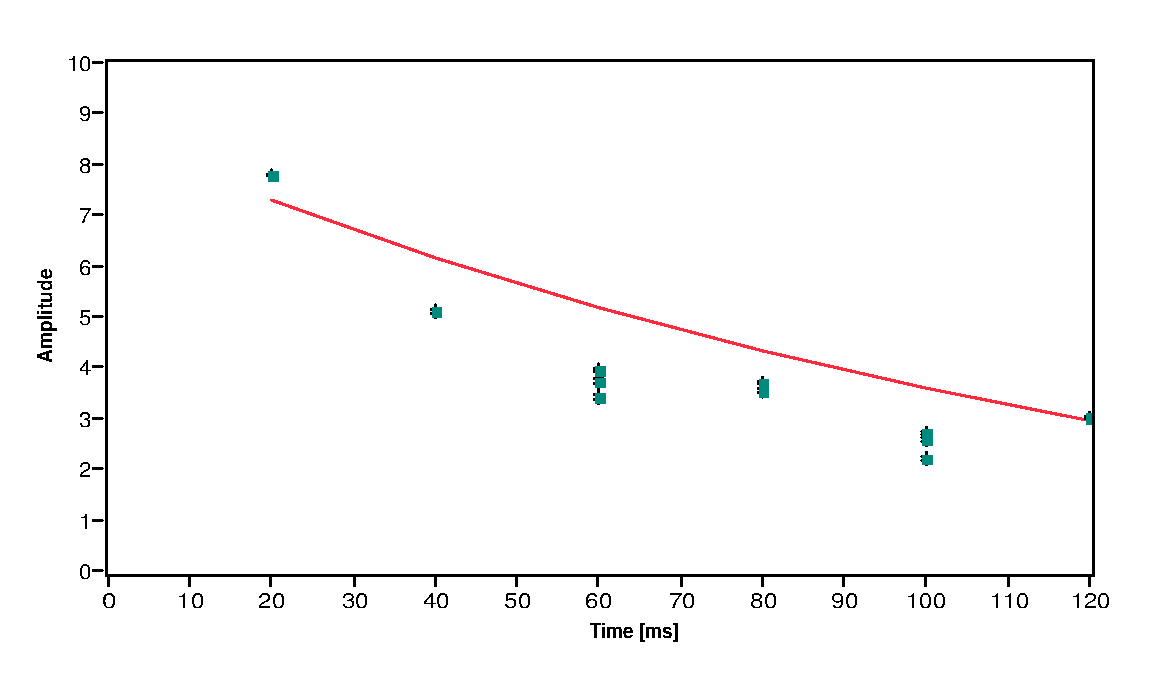
\includegraphics[width=70mm]{./Resources/t2_meas_p1.eps}
			\caption{T2-Measurement Sample 1 with fit.}
			\label{fig:t2_p1}
		\end{figure}
	\end{minipage}
	\hfill
	\begin{minipage}[t]{0.45\textwidth}
		\centering
		\begin{figure}
			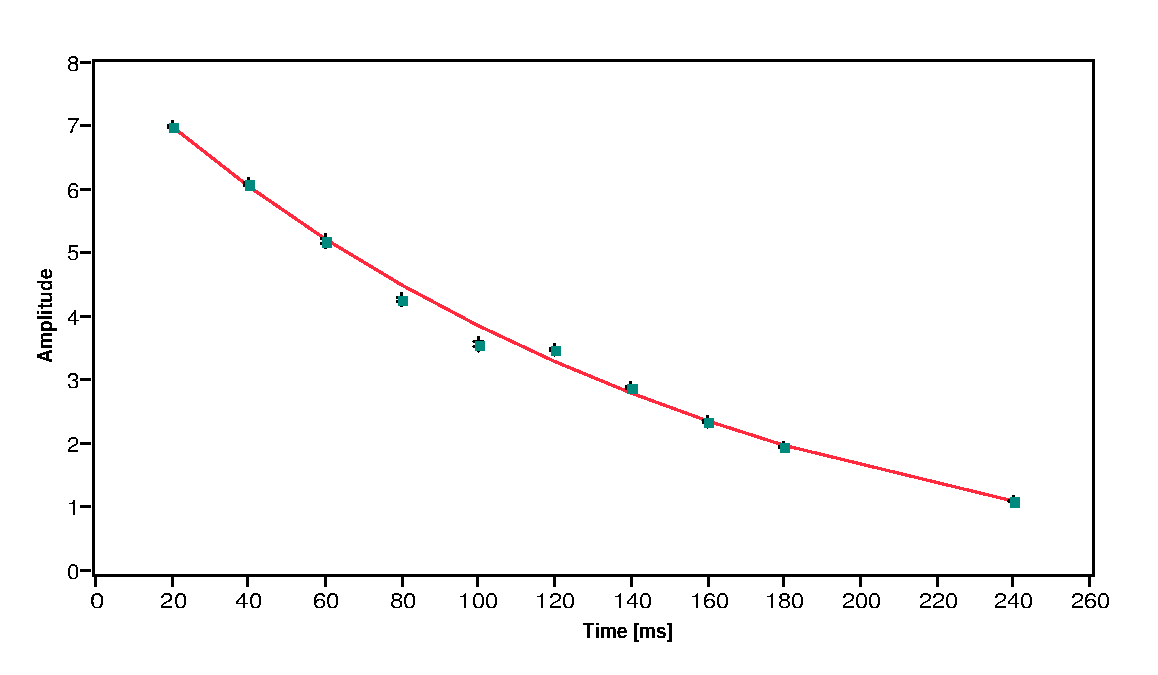
\includegraphics[width=70mm]{./Resources/t2_meas_p3.eps}
			\caption{T2-Measurement Sample 3 with fit.}
			\label{fig:t2_p3}
		\end{figure}
	\end{minipage}
\end{frame}

\begin{frame}
	\frametitle{$T_2$-Measurement: Carr-Purcell Sequence}
	\textbf{Improve dephasing problem of spin-echo method:}
	\begin{itemize}
		\item Inject a $180^\circ$-Pulse on odd multiples of a time $\tau$.
		\item The system is phase coherent on even multiples of a time $\tau$.
	\end{itemize}
	\pause
	\begin{minipage}[t]{0.45\textwidth}
		\centering
		\begin{figure}
			\includegraphics[width=60mm]{./Resources/t2_p1_cp.eps}
			\caption{T2-Measurement using Carr-Purcell, Sample 1, with fit.}
			\label{fig:t2_p1_cp}
		\end{figure}
	\end{minipage}
	\hfill
	\begin{minipage}[t]{0.45\textwidth}
		\centering
		\begin{figure}
			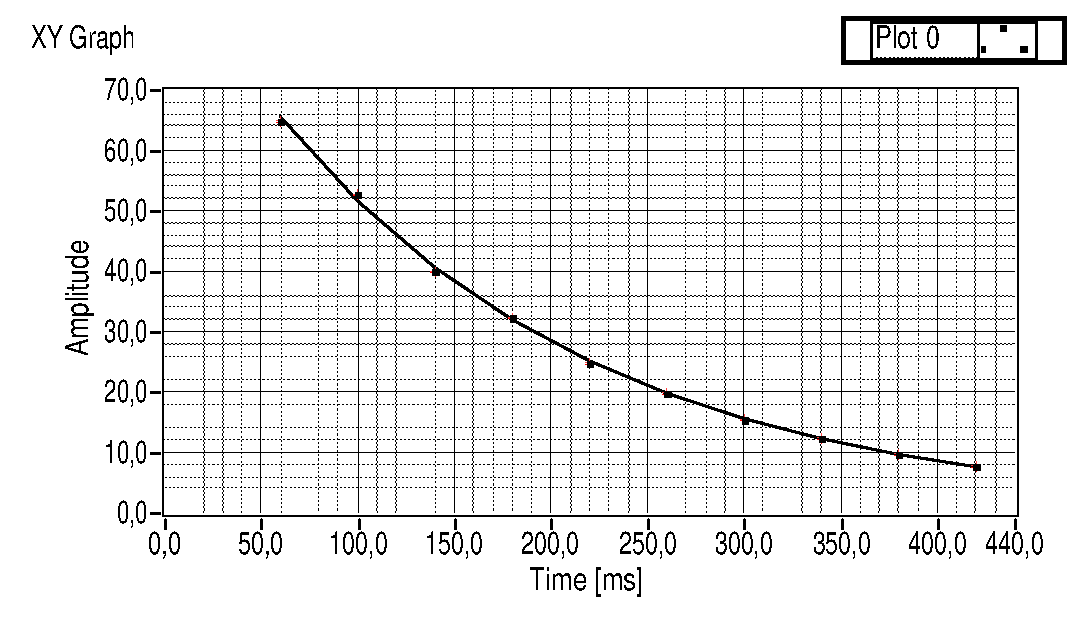
\includegraphics[width=60mm]{./Resources/t2_p3_cp.eps}
			\caption{T2-Measurement using Carr-Purcell, Sample 3, with fit.}
			\label{fig:t2_p3_cp}
		\end{figure}
	\end{minipage}
\end{frame}

\begin{frame}
	\frametitle{$T_1$-Measurement: Spin Echo}
	\textbf{Spin-Echo, but start with a $180^\circ$-Pulse (Anti-parallel Magnetization)}
	\pause
	\begin{minipage}[t]{0.45\textwidth}
		\centering
		\begin{figure}
			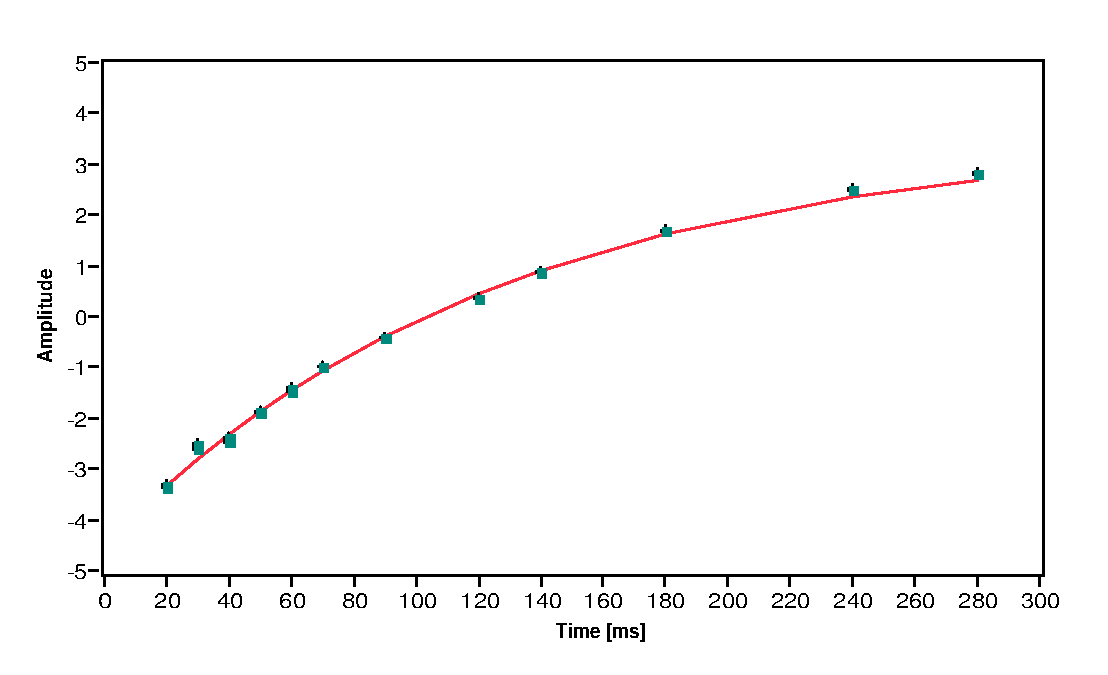
\includegraphics[width=70mm]{./Resources/t1_meas_p1.eps}
			\caption{T1-Measurement Sample 1 with fit.}
			\label{fig:t1_p1}
		\end{figure}
	\end{minipage}
	\hfill
	\begin{minipage}[t]{0.45\textwidth}
		\centering
		\begin{figure}
			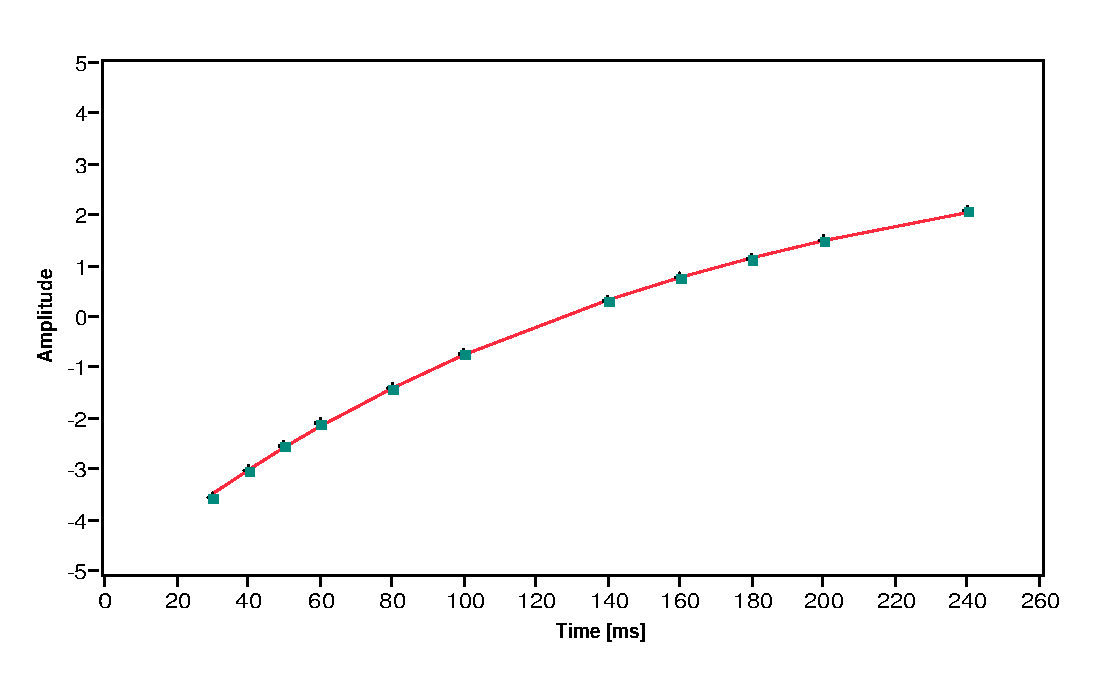
\includegraphics[width=70mm]{./Resources/t1_meas_p3.eps}
			\caption{T1-Measurement Sample 3 with fit.}
			\label{fig:t1_p3}
		\end{figure}
	\end{minipage}
\end{frame}

\begin{frame}
	\frametitle{Relaxation Times: Evaluation}
	\begin{table}[H] 
		\centering
		\caption{Relaxation times -- Measured values}
		\label{tab:relaxtimes}
		\begin{tabular}{cccc}
			\toprule
			Time & $T_1$ [$\mathrm{ms}$] & $T_2$ [$\mathrm{ms}$] & $T_2$ [$\mathrm{ms}$]\\
			Method & Spin-Echo & Spin-Echo & Carr-Purcell\\
			\midrule
			Sample 1 (Gd 1:500)& $\err{125,5}{0,6}$ & $\err{119,5}{0,5}$ & $\err{140,1}{0,4}$\\
			Sample 3 (Gd 1:600)& $\err{150,5}{1,2}$ & $\err{139,3}{0,8}$ & $\err{166,9}{0,4}$\\
			\bottomrule
		\end{tabular}
	\end{table}
	
\end{frame}

\end{document}